\documentclass[a4paper,12pt]{article}
\usepackage[indonesian]{babel}
\usepackage{graphicx}
\usepackage{multirow}
\usepackage{enumitem}
\usepackage{listings}
\usepackage{wrapfig}
\usepackage[T1]{fontenc}
\usepackage{inconsolata}
\usepackage{lipsum}
\usepackage{adjustbox}
\usepackage{upquote}


\usepackage{color}
\usepackage[table]{xcolor}
\definecolor{lightgray}{rgb}{0.95, 0.95, 0.95}
\definecolor{darkgray}{rgb}{0.4, 0.4, 0.4}
%\definecolor{purple}{rgb}{0.65, 0.12, 0.82}
\definecolor{editorGray}{rgb}{0.95, 0.95, 0.95}
\definecolor{editorOcher}{rgb}{1, 0.5, 0} % #FF7F00 -> rgb(239, 169, 0)
\definecolor{editorGreen}{rgb}{0, 0.5, 0} % #007C00 -> rgb(0, 124, 0)
\definecolor{orange}{rgb}{1,0.45,0.13}		
\definecolor{olive}{rgb}{0.17,0.59,0.20}
\definecolor{brown}{rgb}{0.69,0.31,0.31}
\definecolor{purple}{rgb}{0.38,0.18,0.81}
\definecolor{lightblue}{rgb}{0.1,0.57,0.7}
\definecolor{lightred}{rgb}{1,0.4,0.5}
% CSS
\lstdefinelanguage{CSS}{
  keywords={color,background-image:,margin,padding,font,weight,display,position,top,left,right,bottom,list,style,border,size,white,space,min,width, transition:, transform:, transition-property, transition-duration, transition-timing-function},	
  sensitive=true,
  morecomment=[l]{//},
  morecomment=[s]{/*}{*/},
  morestring=[b]',
  morestring=[b]",
  alsoletter={:},
  alsodigit={-}
}

% JavaScript
\lstdefinelanguage{JavaScript}{
  morekeywords={typeof, new, true, false, catch, function, return, null, catch, switch, var, if, in, while, do, else, case, break},
  morecomment=[s]{/*}{*/},
  morecomment=[l]//,
  morestring=[b]",
  morestring=[b]'
}

\lstdefinelanguage{HTML5}{
  language=html,
  sensitive=true,	
  alsoletter={<>=-},	
  morecomment=[s]{<!-}{-->},
  tag=[s],
  otherkeywords={
  % General
  >,
  % Standard tags
	<!DOCTYPE,
  </html, <html, <head, <title, </title, <style, </style, <link, </head, <meta, />,
	% body
	</body, <body,
	% Divs
	</div, <div, </div>, 
	% Paragraphs
	</p, <p, </p>,
	% scripts
	</script, <script,
  % More tags...
  <canvas, /canvas>, <svg, <rect, <animateTransform, </rect>, </svg>, <video, <source, <iframe, </iframe>, </video>, <image, </image>, <header, </header, <article, </article
  },
  ndkeywords={
  % General
  =,
  % HTML attributes
  charset=, src=, id=, width=, height=, style=, type=, rel=, href=,
  % SVG attributes
  fill=, attributeName=, begin=, dur=, from=, to=, poster=, controls=, x=, y=, repeatCount=, xlink:href=,
  % properties
  margin:, padding:, background-image:, border:, top:, left:, position:, width:, height:, margin-top:, margin-bottom:, font-size:, line-height:,
	% CSS3 properties
  transform:, -moz-transform:, -webkit-transform:,
  animation:, -webkit-animation:,
  transition:,  transition-duration:, transition-property:, transition-timing-function:,
  }
}

\lstdefinestyle{htmlcssjs} {%
  % General design
%  backgroundcolor=\color{editorGray},
  basicstyle={\footnotesize\ttfamily},   
  frame=single,
  % line-numbers
  % Code design
  identifierstyle=\color{black},
  keywordstyle=\color{blue}\bfseries,
  ndkeywordstyle=\color{editorGreen}\bfseries,
  stringstyle=\color{editorOcher}\ttfamily,
  commentstyle=\color{brown}\ttfamily,
  % Code
  language=HTML5,
  alsolanguage=JavaScript,
  alsodigit={.:;},	
  tabsize=2,
  showtabs=false,
  showspaces=false,
  showstringspaces=false,
  extendedchars=true,
  breaklines=true,
  % German umlauts
  literate=%
  {Ö}{{\"O}}1
  {Ä}{{\"A}}1
  {Ü}{{\"U}}1
  {ß}{{\ss}}1
  {ü}{{\"u}}1
  {ä}{{\"a}}1
  {ö}{{\"o}}1
}
%
\lstdefinestyle{py} {%
language=python,
literate=%
*{0}{{{\color{lightred}0}}}1
{1}{{{\color{lightred}1}}}1
{2}{{{\color{lightred}2}}}1
{3}{{{\color{lightred}3}}}1
{4}{{{\color{lightred}4}}}1
{5}{{{\color{lightred}5}}}1
{6}{{{\color{lightred}6}}}1
{7}{{{\color{lightred}7}}}1
{8}{{{\color{lightred}8}}}1
{9}{{{\color{lightred}9}}}1,
basicstyle=\footnotesize\ttfamily, % Standardschrift
numbers=left,               % Ort der Zeilennummern
%numberstyle=\tiny,          % Stil der Zeilennummern
%stepnumber=2,               % Abstand zwischen den Zeilennummern
numbersep=5pt,              % Abstand der Nummern zum Text
tabsize=4,                  % Groesse von Tabs
extendedchars=true,         %
breaklines=true,            % Zeilen werden Umgebrochen
keywordstyle=\color{blue}\bfseries,
frame=b,
commentstyle=\color{brown}\itshape,
stringstyle=\color{editorOcher}\ttfamily, % Farbe der String
showspaces=false,           % Leerzeichen anzeigen ?
showtabs=false,             % Tabs anzeigen ?
xleftmargin=17pt,
framexleftmargin=17pt,
framexrightmargin=5pt,
framexbottommargin=4pt,
%backgroundcolor=\color{lightgray},
showstringspaces=false,      % Leerzeichen in Strings anzeigen ?
}%
%
\definecolor{dkgreen}{rgb}{0,.6,0}
\definecolor{dkblue}{rgb}{0,0,.6}
\definecolor{dkyellow}{cmyk}{0,0,.8,.3}

\lstdefinestyle{PHP}{
  language        = php,
  basicstyle      = \small\ttfamily,
  keywordstyle    = \color{dkblue},
  stringstyle     = \color{red},
  identifierstyle = \color{dkgreen},
  commentstyle    = \color{gray},
  emph            =[1]{php},
  emphstyle       =[1]\color{black},
  emph            =[2]{if,and,or,else},
  emphstyle       =[2]\color{dkyellow}}
\lstset{
    showstringspaces=false,
    frame=single,
    breaklines=true,
    rulecolor=\color{black}
}
%

\graphicspath{ {./img/} }
\begin{document}
\title{ {\Large Laporan Praktikum}\\ Pemrograman Web Client\\{\Large Pertemuan 7}}

\author{Aldzikri Dwijayanto Prathama 
	\\195410189
	\\Informatika}
\makeatletter
\begin{titlepage}
	\begin{center}
		{\huge \bfseries \@title }\\[14ex]
		
\includegraphics[scale=.8]{logo}\\[4ex]
		{\large \@author}\\[12ex]
		{\large \bfseries {SEKOLAH TINGGI MANAJEMEN INFORMATIKA DAN KOMPUTER
				AKAKOM YOGYAKARTA}}
	\end{center}


%{\large \@date} 
\end{titlepage}
\makeatother
%\maketitle
\renewcommand{\figurename}{Gambar}
\newpage
\tableofcontents
\newpage
\section{Tujuan}
\begin{enumerate}
    \item Menuliskan script HTML element tabel (table, tr, th, td, tbody, thead, tfoot)
    \item Menuliskan script HTMLelement tabel dan atribut untuk mengatur format tabel (mengabung sel dan membagi sel)
    \item Menuliskan script HTML dan CSS untuk mengatur layout tabel
\end{enumerate}
\section{Dasar Teori}
Tabel merupakan elemen HTML yang mengatur suatu tampilan dalam bentuk kolom
dan baris. Penyajian data dengan menggunakan tabel akan terlihat lebih rapi karena
tersusun secara teratur dalam urutan kolom atau baris. Tag yang digunakan di elemen
tabel adalah:
\begin{table}[!ht]
\begin{tabular}{|l|l|}
\hline
\textless{}table\textgreater{} & Membuat table
\\ \hline
\textless{}th\textgreater{}    & Singkatan table Header untuk membuat header.                                                                                  \\ \hline
\textless{}tr\textgreater{}    & Singkatan table row untuk membuat baris baru.                                                                                 \\ \hline
\textless{}td\textgreater{}    & Singkatan table data untuk menginputkan data .                                                                                \\ \hline
\textless{}thead\textgreater{} & \begin{tabular}[c]{@{}l@{}}Singkatan table head untuk mengelompokkan \\ bagian header.\end{tabular}                           \\ \hline
\textless{}tbody\textgreater{} & \begin{tabular}[c]{@{}l@{}}Singkatan table body untuk mengelompokkan \\ bagian body yang berisi data-data tabel.\end{tabular} \\ \hline
\textless{}tfoot\textgreater{} & Singkatan table footer untuk mengelompokkan bagian footer.                                                                    \\ \hline
\end{tabular}
\end{table}

Penggabungan kolom menggunakan perintah COLSPAN, sedangkan penggabungan baris menggunakan ROWSPAN\@.

\newpage

\section{Pembahasan}
\subsection{Praktik}
\subsubsection{Praktik 1}
Pada praktik pertama adalah membuat tabel menggunakan html, yang berisikan data diri dari empat orang.
\begin{lstlisting}[style=htmlcssjs]
<!DOCTYPE html>
<html>
    <body>
        <table border="1">
            <thead>
                <tr>
                    <th>Nama</th>
                    <th>Kota Asal</th>
                    <th>Umur</th>
                </tr>
            </thead>

            <tbody>
                <tr>
                    <td>Andre</td>
                    <td>Yogyakarta</td>
                    <td>19th</td>
                </tr>
                
                <tr>
                    <td>Susan</td>
                    <td>Bantul</td>
                    <td>20th</td>
                </tr>
                
                <tr>
                    <td>Hartono</td>
                    <td>Bantul</td>
                    <td>19th</td>
                </tr>
                
                <tr>
                    <td>Susanti</td>
                    <td>Klaten</td>
                    <td>19th</td>
                </tr>
            </tbody>

            <tfoot>
                <tr>
                    <td colspan="3">Jumlah Data:4 record</td>
                </tr>
            </tfoot>

        </table>
    </body>
</html>
\end{lstlisting}

Pada dokumen html tersebut terdapat beberapa tag. Tag <table> berfungsi untuk membuat tabel. Tag <thead> berfungsi untuk
mengelompokkan bagian header pada kolom. Tag <th> berfungsi untuk membuat header. Tag <tbody> berfungsi untuk
mengelompokkan bagian-bagian body yang berisi data-data header. Tag <td> berfungsi untuk menginputkan data. Lalu pada
bagian bawah terdapat tag <tfoot> yang berfungsi untuk mengelompokkan bagian footer, di dalamnya terdapat tag <td
colspan=''3''> yabg berfungsi untuk menyatukan 3 kolom.

Setelah dokumen html disave lalu dibuka pada browser, maka tampilannya seperti berikut:
\begin{center}
    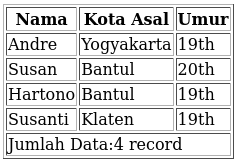
\includegraphics[scale=.7]{1.png} 
\end{center}

\subsubsection{Praktik 2}
Praktik 2 adalah menggabungkan baris dan kolom dengan rowspan dan colspan
\begin{lstlisting}[style=htmlcssjs]
<!DOCTYPE html>
<html>
    <body>

        <table border="1">
            <tr>
                <th>Nama: </th>
                <td>Susanti</td>
            </tr>
            <tr>
                <th rowspan="2">Telp (Kantor & Hp) :</th>
                <td>(0274)555-666</td>
            </tr>
            <tr>
                <td>0877-333-444-555</td>
            </tr>
        </table>

    </body>
</html>
\end{lstlisting}
Untuk menggabungkan 2 baris menjadi 1 baris pada tabel, gunakan tag rowspan="2". Jika dokumen html dibuka pada browser
maka akan nampak seperti berikut:
\begin{center}
    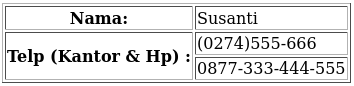
\includegraphics[scale=.7]{2.png} 
\end{center}

\begin{lstlisting}[style=htmlcssjs]
<!DOCTYPE html>
<html>
    <body>
        
        <table border="1">
            <tr>
                <th>Nama</th>
                <th colspan="2">Telp (Kantor & Hp) :</th>
            </tr>
            <tr>
                <td>Susanti</td>
                <td>(0274)555-666</td>
                <td>0877-333-444-555</td>
            </tr>
        </table>

    </body>
</html>
\end{lstlisting}

Sedangkan untuk menggabungkan 2 kolom menjadi satu gunakan tag colspan="2"

\begin{center}
    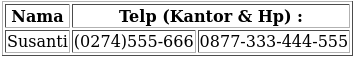
\includegraphics[scale=.7]{3.png} 
\end{center}

\subsubsection{Praktik 3}
Mengatur tampilan tabel dengan css
\begin{lstlisting} 
table {
    font-family: Arial;
    border: 1px solid;
    border-collapse: collapse;
}

td, th {
    border: 1px solid;
    padding: 8px;
}

tr:nth-child(even){background-color:yellow;}
tr:hover{background-color: Red;}
th {
    padding-top: 12px;
    padding-bottom: 12px;
    text-align: left;
    background-color: green;
    color: white;
}
\end{lstlisting}

Pada file CSS tersebut table diatur agar menggunakan font arial, border ukuran 1 pixel. Tag td dan th diatur agar
menggunakan border solid setebal 1px, dan padding 8px. Tag th diatur agar padding atas dan bawah sebesar 12px, text
align ke kiri, warna background hijau, dan warna putih.

\begin{center}
    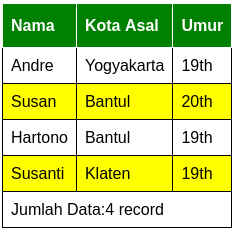
\includegraphics[scale=.7]{4.png} 
\end{center}

\newpage

\subsection{Latihan}
Untuk latihan mahasiswa diminta untuk menampahkan dua baris data baru pada tabel di praktik 1.
\begin{lstlisting}[style=htmlcssjs]
<!DOCTYPE html>
<html>
    <body>
        <table border="1">
            <thead>
                <tr>
                    <th>Nama</th>
                    <th>Kota Asal</th>
                    <th>Umur</th>
                </tr>
            </thead>

            <tbody>
                <tr>
                    <td>Andre</td>
                    <td>Yogyakarta</td>
                    <td>19th</td>
                </tr>
                
                <tr>
                    <td>Susan</td>
                    <td>Bantul</td>
                    <td>20th</td>
                </tr>
                
                <tr>
                    <td>Hartono</td>
                    <td>Bantul</td>
                    <td>19th</td>
                </tr>
                
                <tr>
                    <td>Susanti</td>
                    <td>Klaten</td>
                    <td>19th</td>
                </tr>

                <tr>
                    <td>Budi</td>
                    <td>Jakarta</td>
                    <td>19th</td>
                </tr>

                <tr>
                    <td>Ucup</td>
                    <td>Bandung</td>
                    <td>19th</td>
                </tr>
            </tbody>

            <tfoot>
                <tr>
                    <td colspan="3">Jumlah Data:6 record</td>
                </tr>
            </tfoot>

        </table>
    </body>
</html>
\end{lstlisting}

Untuk menambahkan dua baris data baru pada tabel praktik 1, buat tag <tr> kemudian data dimasukkan pada tag <td>.

\begin{center}
    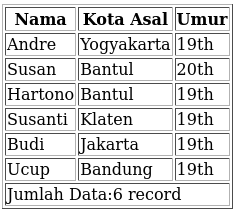
\includegraphics[scale=.7]{5.png} 
\end{center}

\newpage

\section{Kesimpulan}
Setelah praktik ini mahasiswa mampu menuliskan script HTML element tabel (table, tr, th, td, tbody, thead, tfoot),
script HTML element tabel dan atribut untuk mengatur format tabel (mengabung sel dan membagi sel), script HTML dan CSS
untuk mengatur layout tabel

\end{document}
